\chapter{Sensitivity Analysis} \label{ch:sa}

% - why deterministic
%     --> what is stochastic and why we can treat it as deterministic:
%         - stochasticity in the population synthesis
%         - stochasticity in the boarding priority (negligible)

% - borgonovo protocol
%         - outputs
%         - goal
%         - elements
%         - methods
%         - values
%         - visualization
        
% - visualizations & results & comments vari 
After having defined the concepts of Sensitivity Analysis and Agent-based model, and presented my model for the public transportation network in Milan, in this chapter I will proceed to carry out its sensitivity analysis. In particular, in Section \ref{sec:ch4_pre}, I will state the assumptions I make about the model structure, which will allow conducting a smoother investigation. Then, in Section \ref{sec:ch4_steps}, I will present the design of my sensitivity analysis, following the protocol by \textcite{Borgonovo2022SensitivityAO}, and I will conclude in Section \ref{sec:ch4_res} with the results and visualizations.

%%%%%%%%%%%%%%%%%%%%%%%%%%%%%%%%%%%%%%%%%%%%%%%%%%%%%%%%%%%%%%%%%%%%%%%%%%%%%%%%%%%%%%%

\section{Preliminaries} \label{sec:ch4_pre}

The first thing to understand in order to set up the sensitivity analysis of an agent-based model is whether the model under study is stochastic or deterministic. Let us recall the difference between the two frameworks: a model is \textit{deterministic}, if by fixing its input, the output remains unchanged when evaluating the model multiple times; alternatively, a model is \textit{stochastic} if it produces a random value any time it is run with the same fixed input. The nature of the model dictates the kind of output one is going to investigate and the course of the analysis to perform. In the case of a stochastic model, one would want to compute descriptive statistics of the conditional distribution of the output given the fixed values of the inputs, and this requires to evaluate a sufficient number of samples, in order to average out the random component in the output, making the analysis more computationally expensive. If the model is deterministic, instead, one simulation run per each value of the inputs is enough to be able to assess the variations in the outputs. \\ So, before diving deep into the analysis, let us briefly recap the model under study in this research, which has been explained in detail in Chapter \ref{ch:model}, to understand its nature and plan the next steps of the analysis accordingly. The idea of the model is to reproduce the flow of passengers using Milan's transportation network, in order to evaluate the efficiency of the system.
\begin{figure}
    \centering
    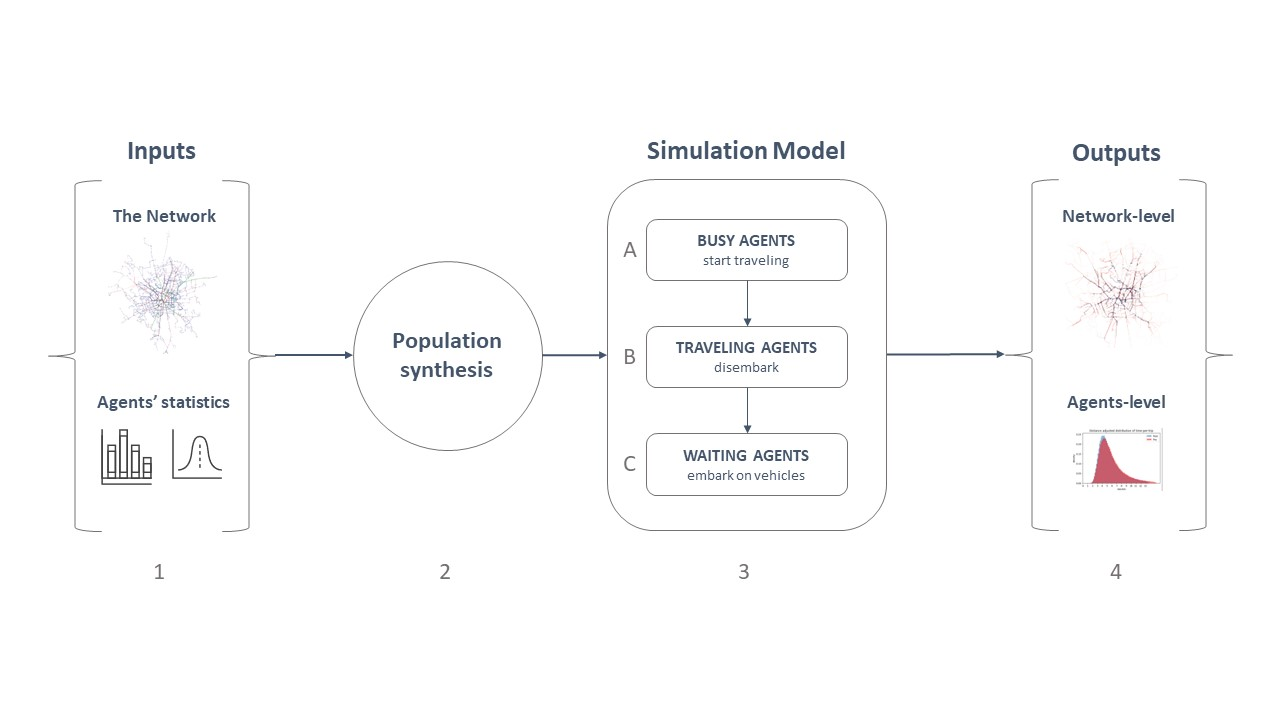
\includegraphics[width = \textwidth]{tex/pics/model_ppt2.jpg}
    \caption{Diagram representing the sequence of steps characterizing the agent-based model under study in this research.}
    \label{fig:model_schema}
\end{figure}
Figure \ref{fig:model_schema} portrays the main phases of the model. On the left side, there are the inputs that need to be fed to the simulator, which can be divided into those needed to construct the network, that will be the environment of the ABM, and those related to the distribution of agents' characteristics. Once one has collected all the inputs, the first step is to run the synthesis of the population. The goal of this phase is to obtain a fictitious population of agents which is as similar as possible to Milan's population, with respect to age, geographical residence and activities performed during an ordinary weekday. Next, the agents obtained are fed, together with the network, to the simulator: as soon as the simulation starts, they begin to move on the network to reach the location of the activities they have to perform. At the end of the simulation, the researcher is able to collect outputs related to the network (e.g. the most overloaded lines) or to the agents (e.g. traveling and waiting time), both at the individual and collective level. 
We can easily recognize two sources of stochasticity in the model's structure:
\begin{itemize}
	\item \textbf{the population synthesis} (2);
	\item \textbf{the boarding priority for waiting agents} (C). 
\end{itemize}
I will now go through each of the two, in order to show that the impact of their stochastic nature on the model's results is negligible. In other words, for the purpose of the sensitivity analysis, from now on we will treat the model as if it were deterministic, that is, as if we obtain the same identical results from each model run, once the network, the population distributions and the number of agents have been fixed. This will allow us to perform one single run for each parameter setting and make the analysis less computationally expensive.

\paragraph{The population synthesis.} 
As described in Section \ref{sec:3.3}, in order to construct the profile of each agent, features like age class, geographical residence and kind of activities performed are drawn from their respective distributions, which have been extrapolated from real demographic data about the residents of Milan. The population synthesis is, thus, a stochastic procedure, producing, at each run, a possibly different sample of agents. The problem with this stochasticity is that agent's behavior in the simulations depends on their characteristics. In particular, the probability of living in a specific zone of the city and that of performing a certain activity are conditional on the age class the agent belongs to, and the number of activities in agents' schedule is among the main drivers of traffic on the network. Moreover, agents' destinations depend on the activity they have to perform, which, again, depends on the age class. In an agent-based model, the results are determined by the collective behavior of agents. Hence, running the simulations with any specific set of individuals would lead to unique results and possibly to the emergence of a distinct phenomenon. For example, in our model, if in a sample the number of agents that have the same destination is above average, then the results of the simulation would be biased, as they could show a particular overload on lines that lead to that specific destination. To eliminate the component in the bias of the results which depends on the population synthesis, a best practice would be to evaluate the model with multiple batches of agents and then average results across simulations. However, one can demonstrate that a large sample size ensures that enough stability in the proportions of the agents' characteristics across different samples is achieved. That is, if the sample size is large enough, then the empirical distribution of agents will resemble the true distribution and one can decide to treat each sample as if they were equivalent, producing the same results. This step can be performed while validating the population synthesis, as to assess its robustness. Indeed, in Section \ref{ssec:3.3.1}, I compared 100 samples of synthetic agents, of which I observed the distributions of multiple characteristics. Results show that, with a sample size of 20000, variability across samples is very low. Hence, I decide to set default sample size to 20000 and disregard the stochasticity in the agents' profiles' creation for the purposes of the sensitivity analysis.

\paragraph{The boarding priority for waiting agents.}
As explained in \ref{sec:3.4}, at each timestep, agents are moved one at a time, and waiting agents are the last to move, as they are allowed to embark on the vehicle only after traveling agents disembarked. While agents having to disembark are always allowed to do so (since there is no capacity constraint associated to stops), those who have to get on a vehicle may be stopped by the constraint that it has already reached full capacity and forced to wait for the next available run. Hence, for waiting agents, the boarding order is important. Indeed, allowing always the same agents to be the first to get on a vehicle would drastically reduce someone's total waiting time and increase someone else's.
In principle, for the purpose of this analysis I am only interested in the collective behavior of agents, and I am not going to inspect agents' individual behavior, as to follow the main scope of the model, that is, evaluating the public transportation system as a whole. So, any boarding priority strategy would be equally valid. However, to be more realistic, I assign the priority with which waiting agents embark on their preferred vehicle at random. 
% More formally, given $c$ the remaining capacity of the vehicle and $w$ the number of waiting agents, we treat each $j$ of the $w$ agents as if they had the same probability of being the $i$-th to embark, for $i = 1, ..., c$, that is, $P[O_j = i] = \frac{1}{c}$, where $O_j$ is the random variable representing the order of embarking for agent $j$. 
Intuitively, given a list of waiting agents, at each timestep the list is randomly shuffled, and the first in the list gets to be the first to move. This is not the only possible strategy. Indeed, one could think of moving agents according to some fixed index, but, as a consequence, the ones with the lowest indices would always be the first to embark and to disembark, exhibiting unrealistically low waiting times, while the opposite would happen for the last agents evaluated. Alternatively, another possibility could be to follow a decreasing order in waiting time, letting the agents arrived earlier at each stop move first. However, this strategy requires making more computations at each timestep, while the adopted strategy seems a reasonable compromise which allows being realistic and avoids giving the first-mover advantage always to the same agents. The problem is that, being this a stochastic strategy, it may happen that running twice the simulation with the same sample of agents would lead to different individual results, meaning the same agent could be waiting more or less across different simulations with identical inputs. Since I am only going to evaluate aggregate results (e.g. mean traveling time, mean waiting time, ...) and neglect individual patterns, I can safely ignore the stochasticity in boarding priority and treat this step as deterministic. Being the boarding procedure the only source of stochasticity left in the simulation model, since we said that the stochasticity in the population synthesis is not significant, we can assume the model has deterministic nature when performing the sensitivity analysis.

%%%%%%%%%%%%%%%%%%%%%%%%%%%%%%%%%%%%%%%%%%%%%%%%%%%%%%%%%%%%%%%%%%%%%%%%%%%%%%%%%%%%%%%

\section{Sensitivity analysis steps} \label{sec:ch4_steps}
I will now illustrate the design of my sensitivity analysis, following the six-steps protocol in \textcite{Borgonovo2022SensitivityAO}. 
\paragraph{1. Output of interest.}
The first step of the sensitivity analysis design consists in choosing the output or outputs of interest. Having determined that the model under study in this research can be treated as deterministic, its outputs are going to be numerical quantities rather than distributions. Among the possible outputs of resulting from the simulations, I focus my analysis on three of them, which I believe reflect different characteristics of the system:
\begin{itemize}
    \item \textbf{The mean waiting time per destination across agents.} ($mean\_wt$) Waiting time is an indicator of passengers' dissatisfaction: agents waiting less are happier about the system. Thus, although this is clearly an agent-related metric, one can think of it also as an index of the network's efficiency. One would expect that this quantity is affected by changes in the values of different parameters characterizing the network, for example vehicles' perceived speeds: if a vehicle is perceived as faster, then more agents would like to use it, causing overload and, as a consequence, higher mean waiting time. 
    \item \textbf{The mean traveling time per km across trips.} ($mean\_minkm$) During the simulation, I collect the time it takes agents to reach each destination in their schedule and the length in km of the path they traverse. The ratio between these two quantities, aggregated across trips, constitutes an output decision-makers could be interested in. Unlike waiting time, which only depends on lines' timetables and on whether vehicles are full or not, traveling time clearly depends on the distance to travel. Instead, traveling time per km is a measure of agents' satisfaction, and, as a consequence, an index of the network's efficiency.
    \item \textbf{The number of edges being full for more than 30 min in a day.} ($full\_edges$) This is a proxy for network overload, thus a direct measure of the system's efficiency. Indeed, one would like edges, and, in turn, vehicles, to have enough capacity to satisfy passengers' demand. A vehicle being full for more than 30 min (not necessarily continuously) causes dissatisfaction and, in turn, inefficiency of the overall network. I expect this quantity to be affected by changes in the network properties: in particular, adding more edges to the network, that is, adding transportation lines or connections among the existing lines, one would expect a lower network overload.
\end{itemize}
During the simulations, I collect additional interesting quantities, such as the percentage of “finished” agents or the average number of vehicles used by agents in a day. In particular, the first should be close to 1 in a perfectly working system, but that is not always the case in our simulations and one would want to inspect which parameters influence variations in its values. Instead, the average number of vehicles is another indicator of agents' satisfaction, as typically passengers prefer to minimize the number of changes in their path, in order to have a smoother experience. For reasons of space, I decided not to focus on these metrics in my research, but they could be used to perform further analysis in the future.


\paragraph{2. Goal.}
This sensitivity analysis has three main goals:
\begin{enumerate}
    \item \textbf{Factor prioritization and factor fixing}, that is, identifying the main drivers of the output variations, for which a more accurate calibration is needed, and the least influential parameters, which one would like to fix to reduce complexity of the model;
    \item \textbf{Direction of change}, meaning I am interested in the sign of the outputs' variations due to changes of input values, to gather managerial insights;
    \item \textbf{Interaction quantification}, to recognize the effects of variations of the values of multiple parameters at the same time. 
\end{enumerate}


\paragraph{3. Elements.}
% {'foot_r', 'speeds', 'am_counts_df', 'p_long', 'agents_strategy'}
In Section \ref{sec:3.4}, I described the model in terms of the structure proposed by \textcite{Borgonovo2022SensitivityAO}, and, in particular, I highlighted the most relevant parameters and procedures. Among the elements presented, I will vary 3 environment-related parameters, 1 agents-related parameter and 1 procedure:
\begin{itemize}
    \item $\mathbf{r_{foot}}$, the maximum distance (in meters) used to consider two stops as "at walking distance". Setting a higher value for this parameter corresponds to possibly adding more edges to the graph representing the transportation network, making it denser.
    \item \textbf{vehicles' speeds vector}, a vector containing the commercial speeds of the different kinds of means of transport, which represents agents' perception of vehicles' speeds. A change in this parameter does not imply a modification in lines' schedule (i.e. vehicles do not become faster), but only a change in edges' weights, used to compute agents' shortest paths. What truly influences the choice of a specific mean of transport is not the absolute value of its speed, but the relative magnitude with respect to the other means' speeds. Changing the relative sizes, agents' paths may be modified, in favor of solutions that are perceived as more convenient, and that could have an impact on traveling times and agents' experience in general.
    \item $\mathbf{r_{pois}}$, the maximum distance (in meters) used to consider a point of interest as "close" to a stop. 
    \item $\mathbf{p_{long}}$, the probability of agents performing "long" tasks rather than short tasks. When more agents are sampled to perform long tasks, the number of passengers traveling late in the evening, that have to go home after they have finished their last activity, increases. It is interesting to check whether this causes, as expected, a decrease in the percentage of agents who manage to finish their schedule, or if it has an impact on agents' waiting time.
    \item \textbf{travel-diary assignment procedure}. This is a "non-parametric" element represented as a categorical variable with values having no ordinal interpretation.
\end{itemize}
I decide not to vary the capacity of vehicles, which, however, would be interesting from the managerial point of view, since the default values are derived from real data about the vehicles currently used by ATM. Any change to capacities in reality would correspond to a huge investment from the company, which needs to be planned in advance, so this study does not seem to have the highest priority in the sensitivity analysis I am proposing.


\paragraph{4. Sensitivity method/design.}
The analysis performed is going to be local, as I am going to evaluate the model at a few points in the input space. Given the nature of the analysis, the method I adopt is that of \textit{finite differences}, which allows estimating the first-order and higher-order derivatives of the output function with respect to input parameters. 
In particular, let $\textbf{x}^0$ and $\textbf{x}^1$ two d-dimensional vectors of inputs in the two scenarios corresponding to the base case and the alternative case, having all inputs at sensitivity value. Evaluating the model at the two scenarios, one obtains $y^0 = g(\textbf{x}^0)$ and $y^1 = g(\textbf{x}^1)$, producing a shift in the model output $\Delta y = y^1 - y^0$. I am going to decompose $\Delta y$ into the portions attributable to the main effect of single inputs, to the interaction of couples, triplets, etc. Since I consider 5 inputs ($d = 5$), $\Delta y$ can be formally expressed as follows:
\[
\Delta y = \sum_{i = 1}^d \phi_i^{0 \rightarrow 1} + \sum_{i<j} \phi_{i,j}^{0 \rightarrow 1} + \sum_{i<j<k} \phi_{i,j,k}^{0 \rightarrow 1} + \sum_{i<j<k<l} \phi_{i,j,k,l}^{0 \rightarrow 1} + \phi_{1,2,...,5}^{0 \rightarrow 1} ,
\]
where the terms in the equation correspond to main effects and interaction effects:
\begin{align*}
    \phi_i^{0 \rightarrow 1} &= g(x_i^1 : \mathbf{x}_{-i}^1) - g(\mathbf{x}^0) , \\
    \phi_{i,j}^{0 \rightarrow 1} &= g(x_{i,j}^1 : \mathbf{x}_{-\{i,j\}}^1) - g(\mathbf{x}^0) - \phi_i^{0 \rightarrow 1} - \phi_j^{0 \rightarrow 1} , \\
    \phi_{i,j,k}^{0 \rightarrow 1} &= g(x_{i,j,k}^1 : \mathbf{x}_{-\{i,j,k\}}^1) - g(\mathbf{x}^0) - \sum_{a<b \in \{i,j,k\}} \phi_{a,b}^{0 \rightarrow 1} - \sum_{a \in \{i,j,k\}} \phi_a^{0 \rightarrow 1} 
\end{align*}
\begin{align*}
    \phi_{i,j,k,l}^{0 \rightarrow 1} &= g(x_{i,j,k,l}^1 : \mathbf{x}_{-\{i,j,k,l\}}^1) - g(\mathbf{x}^0) - \sum_{\substack{a<b<c \\\in \{i,j,k,l\}}} \phi_{a,b,c}^{0 \rightarrow 1} - \sum_{a<b \in \{i,j,k,l\}} \phi_{a,b}^{0 \rightarrow 1} - \sum_{a \in \{i,j,k,l\}} \phi_a^{0 \rightarrow 1} \\
    \phi_{1,2,...,5}^{0 \rightarrow 1} &= g(\mathbf{x}^1) - g(\mathbf{x}^0) - \sum_{\substack{a<b<c<d \\\in \{1,2,...,5\}}} \phi_{a,b,c}^{0 \rightarrow 1} - \sum_{\substack{a<b<c \\\in \{1,2,...,5\}}} \phi_{a,b,c}^{0 \rightarrow 1} - \sum_{a<b \in \{1,2,...,5\}} \phi_{a,b}^{0 \rightarrow 1} - \sum_{a \in \{1,2,...,5\}} \phi_a^{0 \rightarrow 1}
\end{align*}
and the notation $(x_i^1 : \mathbf{x}_{-i}^1)$ indicates the point in the input space in which $x_i$'s value is at the sensitivity case, while all other inputs' values are at the base case.
I am also going to compute the \textit{total finite change effect} of each input $x_i$, that is the fraction of $\Delta y$ attributable to input $x_i$, represented by the sum of all the terms in the decomposition of $\Delta y$ containing index $i$:
\[
\tau_i^{0 \rightarrow 1} =  \phi_i^{0 \rightarrow 1} + \sum_{j \neq i}  \phi_{i,j}^{0 \rightarrow 1} + \cdots + \phi_{1,...5}^{0 \rightarrow 1}.
\]
In order to be able to compute the total finite change effect of each input, it is necessary to evaluate the model at all vertices of 
the hypercube joining $\textbf{x}^0$ and $\textbf{x}^1$, that is, considering a full factorial design between the base case and the sensitivity case. \\
I am going to use \textit{total effects} to answer the factor prioritization goal, while main and interaction effects to address direction of change and interaction quantification.


\paragraph{5. Assignment of values.}
% {'foot_r': 100/200, 'speeds' : 1/2, 'am_counts_df' : 200/500, 'p_long' : 0.7/0.56/0.5, 'agents_strategy' : 1/2}
% speeds_1 = {1: 32, 2: 32, 3: 32, 4: 32, 5: 32, 'TRAM': 11, 'BUS': 14, 'FILOBUS': 14, 'foot': 5}
% speeds_2 = {1: 32, 2: 32, 3: 32, 4: 32, 5: 32, 'TRAM': 14, 'BUS': 14, 'FILOBUS': 14, 'foot': 5} 
I assign two possible values (a \textit{base case} and an \textit{alternative scenario}) to all parameters and procedure except $p_{long}$, for which I provide one \textit{base case} and two \textit{alternative scenarios}. In particular, the values considered are the following:
\begin{itemize}
    \item $\mathbf{r_{foot}}$: two possible values, 100 m, corresponding to a network with 12797 edges, or 200 m, the default value, corresponding to a total of 18470 edges (5673 additional walking paths). Higher values for this parameter are not considered since they would generate a network with a too high number of edges, making shortest-path computations extremely expensive.
    \item \textbf{vehicles' speeds vector}: two versions, differing only in the speed of the tram vehicle type. In particular, in the \textit{alternative scenario} ($speeds_2$) the speed of the tram is increased to be equal to the speed of bus and filobus, so that their relative size passes from 11:14 to 1:1 and the tram becomes as convenient as the other two means. The two vectors considered are the following:
            \begin{itemize}
                \item $speeds_1$ = \{metro: 32, tram: 11, bus: 14, filobus: 14, walking: 5\}
                \item $speeds_2$ = \{metro: 32, tram: 14, bus: 14, filobus: 14, walking: 5\}
            \end{itemize}
    \item $\mathbf{r_{pois}}$: two values, 200 m and 500 m (\textit{base case}). 
    \item $\mathbf{p_{long}}$: three values, 0.5 (\textit{alternative scenario} corresponding to equal probability of performing short and long activities), 0.6 (in-between \textit{alternative}) and 0.7 (\textit{base case}).
    \item \textbf{travel-diary assignment procedure}: two possible values, representing the two strategies explained in Section \ref{sec:3.3} (1 for Strategy 1, the default procedure, and 2 for Strategy 2).
\end{itemize}

I am going to consider a full-factorial design, meaning I am going to evaluate all possible combinations of these parameters' values. This results in 48 model evaluations (or \textit{scenarios}). A summary of the elements and values considered is provided in Table \ref{tab:scenarios}. This design generates one base case $\textbf{x}^0$, with all parameter values set to the default case, and two sensitivity cases $\textbf{x}_1^1$ and $\textbf{x}_2^1$, differing only on the value of $p_{long}$. From now on, we will denote $p\_long\_1 = 0.6$ and $p\_long\_1 = 0.5$. 


\begin{table}
    \centering
    \scalebox{0.7}{
    \begin{tabular}{llll}
    \toprule
    Element &  Name &  Element type &  Values \\
    \midrule
    Max distance (m) for walking edges & $r_{foot}$ & Parameter & 100, 200 \\
    Tram speed & $speed$ & Parameter & 11, 14 \\
    Max distance (m) for points of interest & $r_{pois}$ & Parameter & 200, 500 \\
    Probability of "long" tasks & $p_{long}$ & Parameter & 0.5, 0.6, 0.7 \\
    Travel diary assignment strategy & $agents\_strategy$ & Procedure & 1, 2 \\
    \bottomrule
\end{tabular}
}
    \caption{Inputs and values considered for the sensitivity analysis.}
    \label{tab:scenarios}
\end{table}




\paragraph{6. Results visualization.}
I am going to use bar charts and Pareto charts to visualize total effects and interaction effects. As for direction of change, I am going to create Individual Conditional Expectation (ICE) plots. These consist of lines showing the dependence of the model output on a feature changes: each line is created by evaluating the model with all parameters fixed except for the feature of interest, whose value is varied across the input space.


%%%%%%%%%%%%%%%%%%%%%%%%%%%%%%%%%%%%%%%%%%%%%%%%%%%%%%%%%%%%%%%%%%%%%%%%%%%%%%%%%%%%%%%

\section{Results and visualizations} \label{sec:ch4_res}

% - descrizione delle 48 run on average (+ dire che nell'appendix c'è tutto)
% - cosa ho calcolato? main/interactions/total
% - factor prioritization --> total effects (pareto + commento)
% - interaction effects???????
% - direction of change --> ICE plots

I generated all the combinations of parameters' values, to consider of a full-factorial design as described in the previous section, and evaluated the model at each of the 48 obtained scenarios (details about the parameters' values in each scenario can be found in the appendix \ref{tab:values_settings}). Some statistics about the different runs are displayed in Table \ref{tab:summary_runs} (complete values are available in the appendix \ref{tab:runs_tot}). 

\begin{table}[H]
\centering
\scalebox{0.7}{
    \begin{tabular}{lrrrr}
        \toprule
        {} &  Sample Size &  Finished \% &  Mean \# activities &  Mean \# vehicles \\
        \midrule
        50\%  &     20180.00 &        0.96 &               2.28 &             8.75 \\
        mean &     20220.88 &        0.96 &               2.27 &             8.73 \\
        std  &       225.66 &        0.02 &               0.18 &             0.42 \\
        min  &     20000.00 &        0.92 &               2.09 &             8.20 \\
        max  &     20548.00 &        0.98 &               2.46 &             9.40 \\
        \bottomrule
        \end{tabular}}
        \caption{Summary of the 48 model runs.}
    \label{tab:summary_runs}
\end{table}

The sample size seems comparable across runs, with a standard deviation of 1\%. When one wants to capture the effect of changes in a specific parameter, it is crucial to have a stable sample size, as to eliminate the effects in outputs caused by its variation. Indeed, a considerable discrepancy in the size of the population would cause significant differences in traffic, which would influence all outputs. A second thing to notice from Table \ref{tab:summary_runs} is that the percentage of agents who manage to complete their schedule (\textit{finished}) is never below 92\%, which is around 18000 agents. This is a very good result, and it is a sign of the fact that the network is able to satisfy the given agents' needs. Finally, one can see that the 48 runs are stable also in terms of mean number of activities performed by agents and mean number of vehicles used. The values of the outputs for each of the model evaluations are reported in Table \ref{tab:outputs48}. Starting from these figures, I was able to reconstruct the values of \textit{main effects}, \textit{interaction effects} up to fifth-order and \textit{total effects}, which are reported in the appendix \ref{app:fd}. Given the elements and values described in the previous section, I considered two vectors with full sensitivity values:
\begin{itemize}
    \item $\mathbf{x}^1_1$ = \{$r\_foot$ : 100, \textit{tram speed} : 14, $r\_pois$ : 200,$p\_long$: 0.6, \textit{agents strategy} : 2\},
    \item $\mathbf{x}^1_2$ = \{$r\_foot$ : 100, \textit{tram speed} : 14, $r\_pois$ : 200,$p\_long$: 0.5, \textit{agents strategy} : 2\},
\end{itemize}
differing only in the value for $p\_long$. This implies that I compute two batches of every kind of effect, conditioning on whether the sensitivity value for$p\_long$is set to 0.6 or 0.5. 

% \pagebreak
\begin{table}[H]
    \centering
    \scalebox{0.85}{
\begin{tabular}{lccc}
\toprule
{} &  mean\_wt &  mean\_minkm &  full\_edges \\
\midrule
1  &                  28.6 &   28.504367 &          24 \\
2  &                  21.5 &   26.881428 &          16 \\
3  &                  29.0 &   28.276792 &          23 \\
4  &                  21.2 &   27.101414 &          15 \\
5  &                  21.6 &   24.585317 &          22 \\
6  &                  16.9 &   23.281481 &          16 \\
7  &                  21.6 &   24.493362 &          22 \\
8  &                  16.9 &   23.465794 &          15 \\
9  &                  29.7 &   28.525680 &          24 \\
10 &                  21.3 &   27.138844 &          15 \\
11 &                  28.1 &   28.450146 &          24 \\
12 &                  22.6 &   27.309813 &          13 \\
13 &                  22.9 &   24.897053 &          25 \\
14 &                  17.0 &   23.386810 &          16 \\
15 &                  21.3 &   24.483844 &          22 \\
16 &                  16.8 &   23.378981 &          14 \\
17 &                  29.4 &   28.302854 &          26 \\
18 &                  21.9 &   26.930603 &          16 \\
19 &                  29.7 &   28.391049 &          27 \\
20 &                  21.0 &   26.602387 &          13 \\
21 &                  21.7 &   24.621622 &          22 \\
22 &                  17.2 &   23.631307 &          17 \\
23 &                  21.2 &   24.738400 &          19 \\
24 &                  17.0 &   23.430723 &          17 \\
25 &                  31.9 &   28.568215 &          29 \\
26 &                  24.1 &   27.616700 &          20 \\
27 &                  33.4 &   28.893866 &          27 \\
28 &                  23.7 &   27.353909 &          20 \\
29 &                  24.2 &   24.846904 &          26 \\
30 &                  18.7 &   23.734802 &          19 \\
31 &                  23.4 &   24.657351 &          22 \\
32 &                  18.9 &   23.914512 &          17 \\
33 &                  33.6 &   29.021373 &          32 \\
34 &                  24.5 &   27.508775 &          19 \\
35 &                  32.6 &   28.743855 &          29 \\
36 &                  24.6 &   27.514930 &          24 \\
37 &                  24.3 &   24.972310 &          27 \\
38 &                  18.4 &   23.726622 &          17 \\
39 &                  24.1 &   24.821208 &          23 \\
40 &                  18.9 &   24.054557 &          20 \\
41 &                  32.5 &   28.944984 &          31 \\
42 &                  23.8 &   27.379935 &          18 \\
43 &                  32.8 &   28.605463 &          29 \\
44 &                  23.5 &   27.350090 &          22 \\
45 &                  24.0 &   24.836674 &          23 \\
46 &                  18.6 &   23.864140 &          17 \\
47 &                  23.8 &   24.891937 &          27 \\
48 &                  18.6 &   23.835996 &          19 \\
\bottomrule
\end{tabular}
}
    \caption{Output values of the 48 settings considered.}
    \label{tab:outputs48}
\end{table}

\paragraph{Factor Prioritization.}
Figure \ref{fig:factor_prior} displays 6 Pareto charts showing the total finite change effect of each input on each of the three outputs, when $p\_long$ is set at either of the two sensitivity values. It is easy to see that \textit{tram speed} is the parameter which has the lowest influence on every output, and it has even 0 total effect on waiting time when $p\_long$ is set to 0.6. This means that even if agents perceive the tram as fast as other surface means (bus and filobus), their experience is not changing much. As for the mean traveling time per km ($mean\_minkm$), there is high variability across inputs' total effects, with $r\_foot$ being the most influential. This is intuitive, as a change in the value of this parameter determines a variation in the number of walking paths, that is, a modification of the network: agents can choose among more or less routes to reach their destinations, according to the direction of change of $r\_foot$, and this clearly impacts the mean traveling time. Hence, one should pay more attention to gathering data about how far agents are willing to walk to get on a vehicle, in order to close the gap between the model and reality. 
Regarding the other outputs, the ranking of the different parameter changes as we consider $p\_long\_1$ or $p\_long\_2$, suggesting that one should evaluate interaction effects among $p\_long$ and other inputs, in order to have a complete understanding.

%%%% FACTOR PRIORITIZATION
\begin{landscape}
\centering
\hspace{10cm}
\begin{figure}[h]
    \centering
    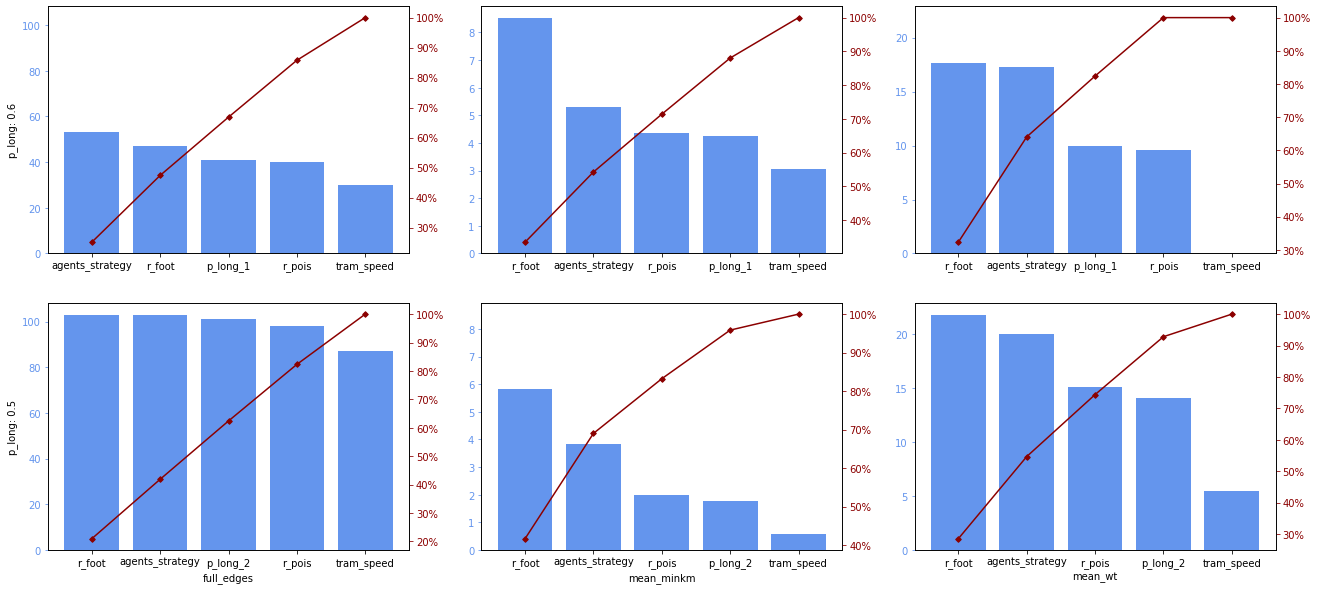
\includegraphics[width = \hsize]{tex/pics/pareto_fp.png}
    \caption{Pareto charts showing the \textit{total finite change effect} of each input with respect to each output, at both sensitivity cases, to answer the goal of factor prioritization.}
    \label{fig:factor_prior}
\end{figure}
\end{landscape}


\paragraph{Direction of Change.}
Figure \ref{fig:ICE} depicts the (ICE) plots for each of the input-output combinations, to be read as follows: for each of the plots, the vertical axis reports the value of the output of the corresponding row (name on the left), conditional on the value of the input of the corresponding column (name at the bottom) in all scenarios. The dots represent the values of the output in a specific run, and each line joins the dots corresponding to the two model evaluations which are conditional on all the other inputs being in the same scenario. The line is colored in \textit{red} if the output value decreases when the parameter value increases, and in \textit{azure} otherwise. I have highlighted in \textit{gray} the vertical line corresponding to the default value for each parameter. From the figure, we can see that changing agents' travel diary assignment procedure from strategy 1 to strategy 2 implies an increase in the value of every output, and we know that higher values of our outputs of interest represent a situation of network inefficiency. This result suggest that, adopting a different sampling strategy, the results obtained lead to different managerial conclusions about the behavior of the system. Hence, to make the model more realistic, one should investigate which of the two strategies portrays reality more accurately. Moreover, it would be interesting to understand which are the direct consequences of assigning activities to the agents with a different algorithm that cause inefficiency of the network. A different case, instead, is that of the \textit{tram speed}: if agents perceive the tram as fast as the other means, then on average they wait less, it takes them less time to traverse 1 km, and the network exhibits a smaller number of edges reaching full capacity for significant amounts of time. As for \textit{r\_foot}, the ICE plots should be read right-to-left, as the base case value is higher than the sensitivity value: in most scenarios, a reduction in the input value produces an increase in outputs, which is intuitive because, if fewer stops are connected between each other, it becomes harder for agents to change vehicle and reach their destinations. However, when it comes to \textit{full\_edges}, there are some scenarios in which the sign of the change following a decrease in \textit{r\_foot} is positive. One should look at the interactions between this input and the others, in order to be able to understand what causes the difference in the behavior of the model.



\paragraph{Interaction effects.} 
I computed all the interaction effects through second up to fifth-order finite difference interactions, and the values are available in the appendix \ref{app:fd}. The tables help to investigate those variations in the outputs which, given a change in an input, do not always go in the same direction in all settings. For example, I already mentioned that, by looking at figure \ref{fig:ICE}, one can notice that in all but a few settings, the outputs increase when $r\_foot$ is set to 100 instead of 200 (negative sign). It turns out that there are two settings in which the total effect is null and only 5 settings in which the opposite happens (positive sign of change). In particular, the steepest increase in $full\_edges$ corresponds to the case in which, together with $r\_foot$, also the \textit{tram speed} and $p\_long$ are at sensitivity cases (the latter is set to 0.5), which is coherent with the fact that the interaction effect among these three parameters is the lowest (-14), as one can see in Table \ref{tab:triplets}. Intuitively, one can think that, although a decrease in $r\_foot$ usually implies more difficulties for agents, the negative effect on the number of edges reaching full capacity for more than 30 min in a day is compensated by the fact that agents perceive the tram as fast as other surface means, and that there is equal probability of performing long and short tasks.

%%%% DIRECTION OF CHANGE
\begin{landscape}
\begin{figure}
    \centering
    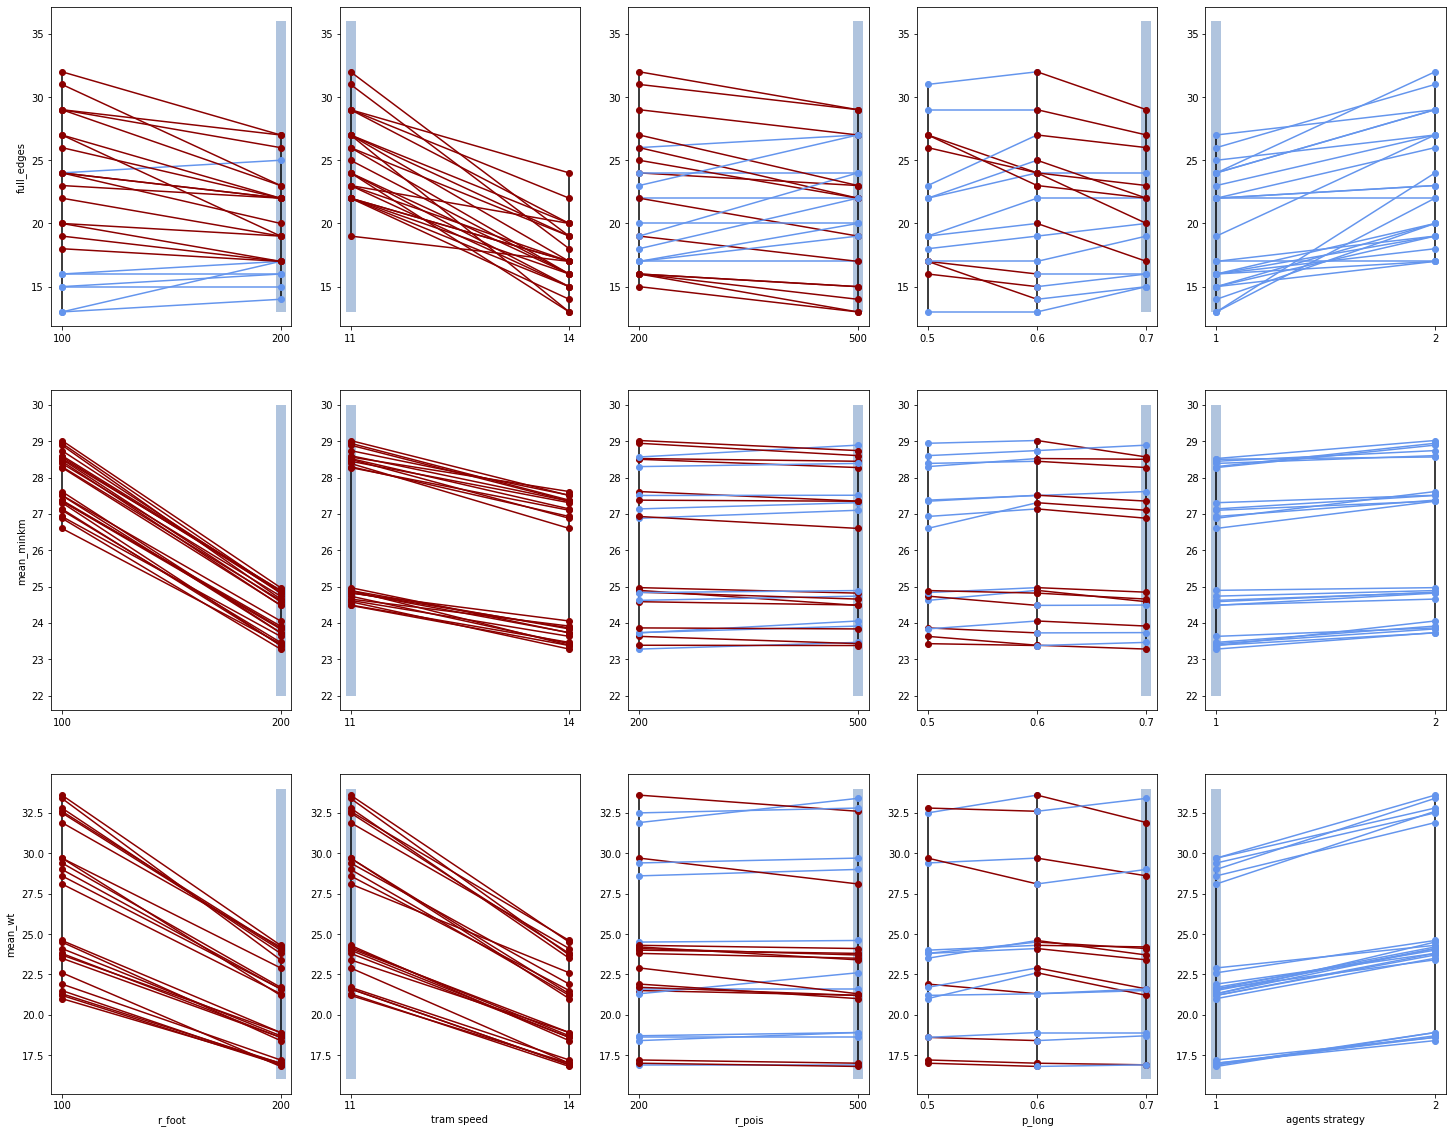
\includegraphics[height = \textheight]{tex/pics/ICE.png}
    \caption{Individual Conditional Expectation (ICE) plots of each input with respect to each output, at both sensitivity cases, to answer the goal of direction of change. Lines are \textit{red} if the output value decreases when the parameter value increases, and \textit{azure} otherwise.}
    \label{fig:ICE}
\end{figure}
\end{landscape}